\section{Zmeny na robote}

\subsection{Pokazený systém}
\label{subsec:brokenSystem}

Prvýkrát, keď sme prišli k robotu do NCR (\acrlong{NCR}), tak sme si určili ako prvú úlohu zálohovať systém. Ak by sa teda stala nejaká chyba
a robot by prestal fungovať, tak by sme sa vedeli dostať do posledného funkčného stavu robota. Zálohovanie systému nanešťastie nebolo možné
hneď po zapnutí robota. Bolo to preto, lebo po tom, ako na robote robili študenti tímový projekt~\cite{timovyProjekt}, tak na robote niekto
stiahol ROS1 (\acrlong{ROS}) verzia \textit{Lunar Loggerhead}. Toto by problém nespôsobilo, čo ale problém spôsobilo, bolo jeho nesprávne odinštalovanie.
Táto akcia mala za dôsledok vypisovanie nasledovnej chybovej hlášky pri zálohovaní.

\begin{lstlisting}
	E: Unable to correct problems, you have held broken packages.
\end{lstlisting}

Tento problém sme vyriešil vymazaním všetkých knižníc, ktoré boli nainštalované spolu s ROS1. Toto vyriešilo problém. Na vymazanie týchto
knižníc sme použili nasledovný príkaz.

\begin{lstlisting}[language=bash]
	sudo apt autoremove && sudo dpkg --remove $(dpkg --get-selections | grep hold)
\end{lstlisting}

Tento príkaz najprv odstráni všetky balíčky, ktoré nie sú používané žiadnou aplikáciu v systéme. Následne vyhľadá všetky knižnice,
ktoré taktiež nie sú používané žiadnym balíčkom a nasilu odinštaluje. Po vykonaní tejto operácie sme ešte museli odstrániť všetky referencie
na ROS1 v~systéme. Toto sme vykonali odstránením linkov na už neaktívne repozitáre, ktoré sa nachádzali v súbore \textit{/etc/apt/sources.list}.

\subsection{Nesprávna funkcia robota}
\label{subsec:wrongFunctionality}

Ako bolo spomenuté vyššie, pri~poslaní príkazu s~číslom~\ref{c6} nám robot vráti aktuálne rýchlosti kolies. Počas skúšania tejto funkcionality
sme narazili na~problém. Keď sme sa robota spýtali na~jeho rýchlosti. Dostali sme reťazec, ktorý obsahoval náhodne veľké čísla. Tieto čísla sa
menili, keď sme zadávali nejaké hodnoty pre~rýchlosti kolies aby~sa robot hýbal. Ich magnitúda ale ostávala nezmenená. V~nasledujúcom príklade
môžeme vidieť ako tento reťazec vyzeral:

\label{jsonWannabeSpeed}
\begin{lstlisting}
		{"LeftWheelSpeed"=236223201280 "RightWheelSpeed"=4294967296}
\end{lstlisting}

Tu vidíme príklad obdržanej správy. Ako si môžeme všimnúť. Pri~tomto type správ nie je dodržaná správna forma reťazca typu \textit{JSON}.
Namiesto `:' máme `=' a~medzi argumentmi sa nenachádza čiarka. Hneď ako prvú vec sme chceli tento štandard napraviť. Bohužiaľ na~tomto
robote už~bolo spravených niekoľko projektov a~museli by sme prejsť každý z~nich a~zistiť či~používajú túto spätnú väzbu. Ak~by ju používali
museli by sme tieto kódy upraviť.

V~dokumentácii robota bohužiaľ nebolo písané v~akom formáte sa tieto rýchlosti kolies majú nachádzať. Preto jeden z~nápadov ako zistiť presne
v~akom formáte sa posielali tieto čísla bolo vyskúšať pár možností. Boli to

\begin{itemize}
	\item \textit{long} - celé číslo s malým endianom
	\item \textit{long} - celé číslo s veľkým endianom
	\item \textit{float} - desatinné číslo s malým endianom
	\item \textit{float} - desatinné číslo s veľkým endianom
\end{itemize}

Keďže robot má počítač so~63 bytovým procesorom \cite{robotPc}, tak~\textit{long} aj~\textit{float} budú mať 64 bitovú dĺžku. Po~skúsení všetkých
štyroch možností sa~ukázalo, že~ani jedna nebola správna a~problém je niekde inde.

Problém je v~tom, že~keď posielame request na~nastavenie rýchlosti kolies, tak~kód na~robote funguje tak, že~si ich premení na~celé čísla v~rozsahu
0~až~1000. To~je hodnota, na~ktorú nastaví rýchlosti otáčania pravého a~ľavého kolesa respektíve rýchlosť otáčania ich motorov. Na~druhú stranu,
keď si vypýtame od~robota rýchlosti kolies. On zoberie informáciu z~enkóderov a~pošle nám ju~bez spracovania. Aj napriek týmto poznatkom sa nám
nepodarilo získať z~týchto dát žiadané rýchlosti.

Po dôkladnom preštudovaní kódu sme zistili, že~hodnoty ktoré nám posiela robot nie sú ani~vyťahované z~enkóderov správnou funkciou. Preto~sme ju
zmenili a~začali sme dostávať hodnoty, s~ktorými by sa mohlo dať pracovať.

Funkcie z~knižnice zabezpečujúce komunikáciu z~enkóderov motorov pochádzajú z~firmy Maxon~\cite{EPOSdoc}. Táto dokumentácia nebola moc nápomocná.
Opisy jednotlivých funkcií boli len~ich rozložené názvy na~osobitné slová. Aj~napriek tomu sa nám podarilo nájsť funkcie, ktoré sme potrebovali.
Funkcie, ktoré končia koncovkou `Target', alebo toto slovo obsahujú, majú návratné hodnoty reprezentujúce žiadané hodnoty. Funkcie s~koncovkou
`Is' vracajú aktuálne hodnoty. Z~tohto dôvodu sme museli prepísať funkciu na~robote, ktorá sa vykonávala, keď sme chceli získať aktuálne hodnoty
rýchlosti motora poslaním príkazu \ref{c6}. Funkciu, ktorú sme zmenili môžeme vidieť v~nasledujúcej ukážke:

\lstset{language=C++,
	basicstyle=\ttfamily,
	keywordstyle=\color{blue}\ttfamily,
	stringstyle=\color{red}\ttfamily,
	commentstyle=\color{green}\ttfamily,
	morecomment=[l][\color{magenta}]{\#},
	numberstyle=\color{orange}
}

\label{VelocityIs}
\begin{lstlisting}[language=C++]
BOOL VCS_GetTargetVelocity(
	HANDLE KeyHandle,
	WORD NodeId,
	long* pTargetVelocity,
	DWORD* pErrorCode);
\end{lstlisting}

\begin{lstlisting}[language=C++]
BOOL VCS_GetVelocityIs(
	HANDLE KeyHandle,
	WORD NodeId,
	long* pVelocityIs,
	DWORD* pErrorCode);
\end{lstlisting}

\noindent Ako môžeme vidieť v~týchto predpisoch funkcií, bolo treba zmeniť názov funkcie a~ostatné parametre ostali rovnaké.
Nebolo treba meniť implementáciu kódu.

\subsection{Zašumený výstup}

Po~prepísaní funkcie na~získavanie rýchlostí robota sme spravili pár meraní, aby sme zistili, aké presné informácie o~rýchlostiach
motorov dostávame. Aby nám robot neodbiehal postavili sme ho na~vyvýšené miesto, tak~aby sa kolesá nedotýkali zeme. V~takomto
postavení sa robot nepohne z~miesta a~my môžeme bez~problémov odmerať prechodové a~prenosové charakteristiky rýchlosti pravého
a~ľavého motora.

\begin{figure}[!htbp]
	\begin{subfigure}{0.5\textwidth}
		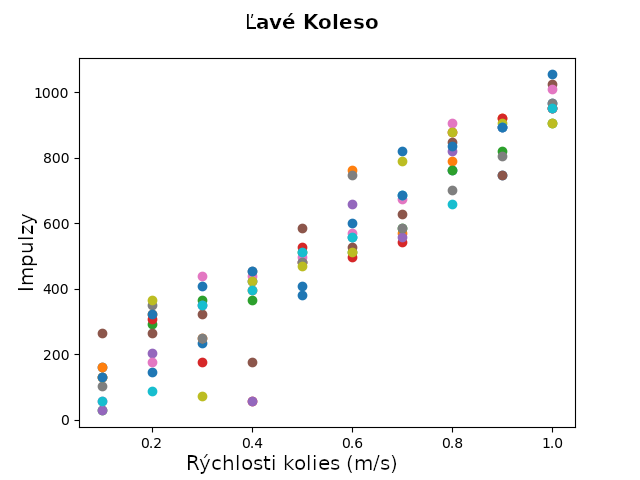
\includegraphics[width=\textwidth]{img/Left_wheel_2.png}
	\end{subfigure}
	\hfill
	\begin{subfigure}{0.5\textwidth}
		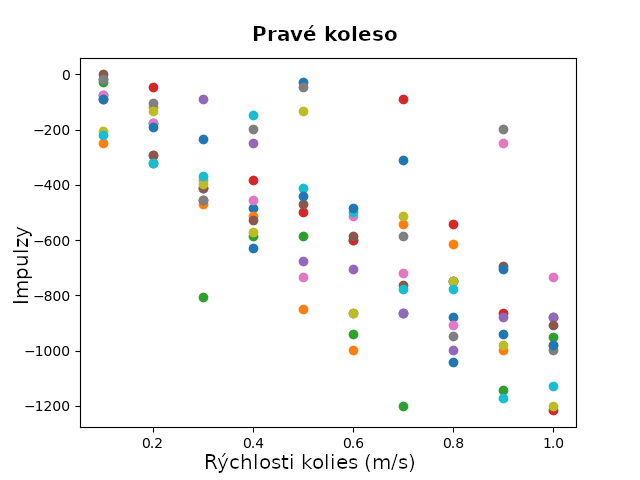
\includegraphics[width=\textwidth]{img/Right_wheel_2.png}
	\end{subfigure}
	\caption{Ustálené hodnoty rýchlosti ľavého a~pravého motora. }
	\label{fig:lavePraveKoleso}
\end{figure}

Po~obdržaní takýchto dát sme kontaktovali jedného z~autorov tímového projektu~\cite{timovyProjekt}, Adriána Kasperkevic. On nám odpísal s~tým,
že~aj oni mali problémy s~enkódermi. Na obrázku Obr.~\ref{fig:prechChar} vidíme zašmený signál rýchlosti poskytovanú enkódermi. Ich problémy
boli naviazané na~staré enkódery, ktoré neskôr vymenili. Na~nových enkodéroch avšak netestovali ich spätnú väzbu.

\begin{figure}[!htbp]
	\begin{center}
		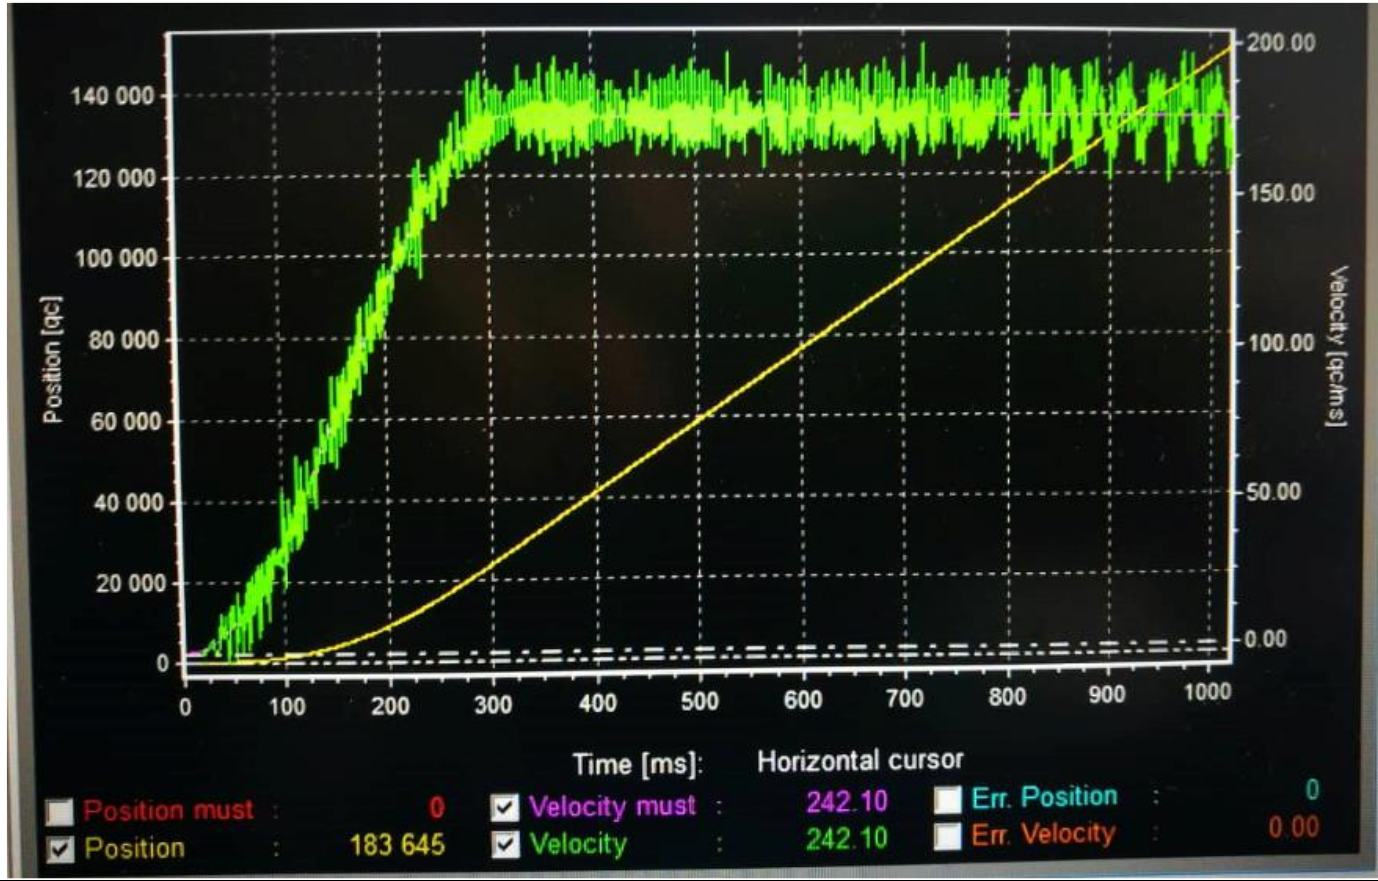
\includegraphics[width=0.95\textwidth]{img/robotSpeedChar.png}
	\end{center}
	\caption{Prechodová charakteristika rýchlosti kolies~\cite{timovyProjekt}. }
	\label{fig:prechChar}
\end{figure}

